\documentclass[a4paper, 11pt, pdftex]{report}
\usepackage{graphicx}
\usepackage{amsmath, amsthm}
\usepackage[T1]{fontenc}
\usepackage[full]{textcomp}
\usepackage[charter]{mathdesign}
\usepackage[utf8]{inputenc}
\usepackage[english]{babel}
%\usepackage[]{showkeys}
\usepackage{hyperref}
\usepackage[all]{hypcap}
\usepackage[noend]{algorithm, algpseudocode}
\usepackage{listingsutf8}
\usepackage{mathtools}
\usepackage[svgnames]{xcolor}
\usepackage{multirow}
\usepackage{enumitem} 

\usepackage{fullpage}
\setlength\parindent{0pt}
\setlength\parskip{\baselineskip}
\setlength{\abovedisplayskip}{0pt}
\sloppy
\pagestyle{plain}

\usepackage{epigraph}
\setlength\epigraphwidth{.65\textwidth}

\theoremstyle{plain}
\newtheorem{theorem}{Theorem}[chapter]
\newtheorem*{theorem*}{Theorem}

\theoremstyle{definition}
\newtheorem{algo}[theorem]{Algorithm}

\usepackage{chngcntr}
\counterwithin{figure}{chapter}
\counterwithin{table}{chapter}

\makeatletter
\renewcommand*{\thetable}{\arabic{chapter}.\arabic{table}}
\renewcommand*{\thefigure}{\arabic{chapter}.\arabic{figure}}
\let\c@table\c@figure
\makeatother 

\DeclareMathOperator{\bit}{bit}
\DeclareMathOperator{\bitRev}{bitRev}
\DeclareMathOperator{\re}{Re}
\DeclareMathOperator{\im}{Im}

\newcommand\T{\rule{0pt}{2.6ex}}
\newcommand\B{\rule[-1.4ex]{0pt}{0pt}} 

\begin{document}

\begin{titlepage}
	\centering
	\vspace*{2cm}
	{\scshape\huge f\textsubscript{12}ecm\par}
	\vspace{2cm}
	{\scshape\Large A program for finding\\the factors of\\the 12\textsuperscript{th} Fermat number\par}
	\vspace{4cm}
	{\huge\bfseries Elliptic Curve Method\\and\\Probabilities\par}
	\vspace{4cm}
	{\Large\itshape Yves Gallot\par}
	\vfill
	{\large \today\par}
\end{titlepage}

\vspace*{2cm}
{\scshape f\textsubscript{12}ecm} is free source code, under the MIT license.

Copyright (c) 2021, Yves Gallot

Permission is hereby granted, free of charge, to any person obtaining a copy
of this software and associated documentation files (the "Software"), to deal
in the Software without restriction, including without limitation the rights
to use, copy, modify, merge, publish, distribute, sublicense, and/or sell
copies of the Software, and to permit persons to whom the Software is
furnished to do so, subject to the following conditions:

The above copyright notice and this permission notice shall be included in
all copies or substantial portions of the Software.

THE SOFTWARE IS PROVIDED "AS IS", WITHOUT WARRANTY OF ANY KIND, EXPRESS OR
IMPLIED, INCLUDING BUT NOT LIMITED TO THE WARRANTIES OF MERCHANTABILITY,
FITNESS FOR A PARTICULAR PURPOSE AND NONINFRINGEMENT. IN NO EVENT SHALL THE
AUTHORS OR COPYRIGHT HOLDERS BE LIABLE FOR ANY CLAIM, DAMAGES OR OTHER
LIABILITY, WHETHER IN AN ACTION OF CONTRACT, TORT OR OTHERWISE, ARISING FROM,
OUT OF OR IN CONNECTION WITH THE SOFTWARE OR THE USE OR OTHER DEALINGS IN
THE SOFTWARE.


\chapter{Introduction}

\epigraph{Si je puis une fois tenir la raison fondamentale que 3, 5, 17, etc. sont nombres premiers,
il me semble que je trouverai de très belles choses en cette matière,}
{\textit{Fermat à Mersenne \\ 25 décembre 1640}}

Pierre de Fermat conjectured that every number of the form $F_{n} = 2^{2^n} + 1,$ where $n$ is a non-negative integer, is prime \cite{Fermat1}. Today these positive integers are named Fermat numbers. The first five Fermat numbers are prime, but Leonhard Euler proved in 1732 that $641$ divides $F_5$.

$F_6$ was completely factored by T~Clausen, F.~Landry and H.~Le~Lasseur in 1855. In 1970, M.~A.~Morrison and J.~Brillhart cracked $F_7$ by the Continued Fraction method \cite{MorrisonBrillhart1}. In 1980, 		R.~P.~Brent and J.~M.~Pollard used a modification of Pollard's rho method to factor $F_8$. R.~P.~Brent completely factored $F_{11}$ in 1988 by ECM \cite{Brent2}. In 1990, A.~K.~Lenstra, H.~W.~Lenstra, M.~S.~Manasse and J.~M.~Pollard organized a distributed computation on approximately 700 workstations around the world and factored $F_9$ by the Number Field Sieve \cite{Lenstra2ManassePollard}. Finally R.~P.~Brent completely factored $F_{10}$ in 1995 by ECM \cite{Brent2}.

The smallest Fermat number which is not completely factored is $F_{12}$. Six prime factors are known, the 54-digit factor was found by Michael Vang in 2010 using GMP--ECM \cite{Vang1}.

\begin{tabular}{lcl}
	\T $F_5$ &= &$641 \:\cdot\: 6700417$\\
	\T $F_6$ &= &$274177 \:\cdot\: 67280421310721$\\
	\T $F_7$ &= &$59649589127497217 \:\cdot\: 5704689200685129054721$\\
	\T $F_8$ &= &$1238926361552897 \:\cdot\: P_{62}$\\
	\T $F_9$ &= &$2424833 \:\cdot\: 7455602825647884208337395736200454918783366342657 \:\cdot\: P_{99}$\\
	\T $F_{10}$ &= &$45592577 \:\cdot\: 6487031809 \:\cdot\: 4659775785220018543264560743076778192897 \:\cdot\: P_{252}$\\
	\T $F_{11}$ &= &$319489 \:\cdot\: 974849 \:\cdot\: 167988556341760475137 \:\cdot\: 3560841906445833920513 \:\cdot\: P_{564}$\\
	& & \\
	\T $F_{12}$ &= &$114689 \:\cdot\: 26017793 \:\cdot\: 63766529 \:\cdot\: 190274191361 \:\cdot\: 1256132134125569 \:\cdot$\\
	 & &$568630647535356955169033410940867804839360742060818433 \:\cdot\: C_{1133}$
\end{tabular}

\chapter{Elliptic curves over finite fields}

\chapter{Elliptic Curve Method}
\section{Implementation}
\section{Probabilities}

Dickman \cite{Dickman1} proved that the probability that a large integer $n$ has no prime factor
exceeding $n^\alpha$ approaches a limit $F(\alpha)$ as $n \to \infty$, where
\begin{equation*}
F(\alpha) = \begin{cases}
1 - \int_\alpha^1 F(\frac{t}{1-t}) \frac{dt}{t} & \text{if } 0 \leq \alpha < 1 \text{,}\\
1& \text{if } \alpha \geq 1 \text{.}
\end{cases}
\end{equation*}

Let $u = 1/\alpha$. $F(1/u) = 1 - \int_{1/u}^1 F(\frac{t}{1-t})\, \frac{dt}{t}$.
If $t' = 1/t$ we have $\frac{t}{1-t} = \frac{1}{t' - 1}$ and $\frac{dt}{t} = -\frac{dt'}{t'}$
then $F(1/u) = 1 - \int_1^u F(\frac{1}{t' - 1}) \frac{dt'}{t'}$. The relation becomes
\begin{equation*}
F(1/u) = \rho(u) = \begin{cases}
1 - \int_1^u \frac{\rho(t - 1)}{t}\, dt & \text{if } u > 1 \text{,}\\
1 & \text{otherwise.}
\end{cases}
\end{equation*}

$\rho$ is the Dickman function used to estimate the proportion of smooth numbers up to a given bound.

Differentiating both sides of the definition of $\rho(u)$ for $u > 1$ gives
$t\, \rho'(t) = -\rho(t - 1)$. Integration by parts of $\rho(t)$ and $t$ is
$\int_1^u \rho(t)\, dt = \left[ t\, \rho(t) \right]_1^u - \int_1^u t\, \rho'(t)\, dt$. Hence
$\int_1^u \rho(t)\, dt = u\, \rho(u) - 1 + \int_0^{u-1} \rho(t) \, dt$. Since
$\int_0^1 \rho(t) \, dt = 1$ we have
$$\rho(u) = \frac{1}{u} \int_{u - 1}^u \rho(t)\, dt.$$

This relation can be used for the numerical computation of $\rho$ by approximating the integral
with the trapezoidal formula \cite{LuneWattel1}. If $1 \leq u < 2$,
$\rho(u) = 1 - \int_1^u \frac{dt}{t} = 1 - \log u$.


Knuth and Trabb Pardo \cite{KnuthPardo1} extended Dickman's theorem and shown that the
probability that the $k^\text{th}$ largest prime factor of a number $n$ is at most $n^\alpha$
tends to a limiting distribution $F_k(\alpha)$ as $n \to \infty$, where $F_0(\alpha) = 0$ for all
$\alpha$ by convention and for $k \geq 1$
\begin{equation*}
F_k(\alpha) = \begin{cases}
1 - \int_\alpha^1 \left( F_k(\frac{t}{1-t}) - F_{k-1}(\frac{t}{1-t}) \right) \frac{dt}{t} & \text{if } 0 \leq \alpha < 1 \text{,}\\
1& \text{if } \alpha \geq 1 \text{.}
\end{cases}
\end{equation*}

We can define the generalized Dickman function $\rho_k(u) = F_k(1/u)$ and we have
\begin{equation*}
\rho_k(u) = \begin{cases}
1 - \int_1^u \left( \rho_k(t - 1) - \rho_{k-1}(t - 1) \right) \frac{dt}{t}
  & \text{if } u > 1 \text{ and } k\geq 1\text{,}\\
1& \text{if } 0 < u \leq 1 \text{ and } k\geq 1\text{,}\\
0& \text{otherwise.}
\end{cases}
\end{equation*}

The differential equation is $t\, \rho'_k(t) = -\rho_k(t - 1) + \rho_{k-1}(t - 1)$.
Integrating by parts, we get
$$\rho_k(u) = \frac{1}{u} \left( \int_{u-1}^u \rho_k(t)\, dt + \int_0^{u-1} \rho_{k-1}(t)\, dt \right).$$
This relation can be used for the numerical computation of $\rho_2$.

\bigskip

\begin{figure}[ht]
	\capstart
	\centering
	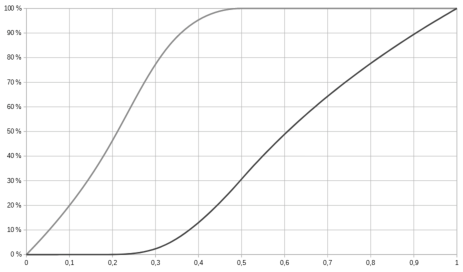
\includegraphics[width=16cm, angle=0]{F_12.pdf}
	\caption{\label{fig:F_12} $F(\alpha)$ and $F_2(\alpha)$.}
\end{figure}


\begin{thebibliography}{99}

\bibitem{Brent1} Richard~P.~Brent, \emph{Factorization of the tenth Fermat number}, Math. Comp. \textbf{68} (1999), 429--451, DOI: \url{https://doi.org/10.1090/S0025-5718-99-00992-8}.

\bibitem{Brent2} Richard~P.~Brent, \emph{Factorization of the tenth and eleventh Fermat numbers}, Report TR-CS-96-02, Computer Sciences Laboratory, Australian National Univ., Canberra, Feb. 1996, \url{https://citeseerx.ist.psu.edu/viewdoc/download?doi=10.1.1.70.6415&rep=rep1&type=pdf}.

\bibitem{BrentPollard1} Richard~P.~Brent and John~M.~Pollard, \emph{Factorization of the eighth Fermat number}, Math. Comp. \textbf{36} (1981), 627--630, DOI: \url{https://doi.org/10.1090/S0025-5718-1981-0606520-5}.

\bibitem{Dickman1} Karl~Dickman, \emph{On the Frequency of Numbers Containing Prime Factors of a Certain Relative Magnitude}, Arkiv för Mat., Astron. och Fys. 22A, 1-14, 1930. 

\bibitem{Fermat1} Pierre~de~Fermat, \emph{Lettre à Marin Mersenne}, \url{https://www.archive.org/stream/oeuvresdefermat942ferm#page/212/mode/2up}.

\bibitem{KnuthPardo1} Donald~E.~Knuth and Luis~Trabb~Pardo, \emph{Analysis of a simple factorization algorithm}, Theoretical Computer Science, Volume 3, Issue 3, December 1976, Pages 321--348, DOI: \url{https://doi.org/10.1016/0304-3975(76)90050-5}.

\bibitem{Lenstra2ManassePollard} A.~K.~Lenstra, H.~W.~Lenstra, M.~S.~Manasse and J.~M.~Pollard, \emph{The factorization of the ninth Fermat number}, Math. Comp. \textbf{61} (1993), 319--349, DOI: \url{https://doi.org/10.1090/S0025-5718-1993-1182953-4}.

\bibitem{LuneWattel1} J.~van~de~Lune and E.~Wattel, \emph{On the numerical solution of a differential-difference equation arising in analytic number theory}, Math. Comp. \textbf{23} (1969), 417--421, DOI: \url{https://doi.org/10.1090/S0025-5718-1969-0247789-3}.

\bibitem{MorrisonBrillhart1} Michael~A.~Morrison and John~Brillhart, \emph{A method of factoring and the factorization of $F_7$}, Math. Comp. \textbf{29} (1975), 183--205, DOI: \url{https://doi.org/10.1090/S0025-5718-1975-0371800-5}.

\bibitem{Vang1} \url{https://caramel.loria.fr/f12.txt}.

\end{thebibliography}

\end{document} 
